\documentclass[tikz,border=3pt]{standalone}
\usetikzlibrary{calc}
\usetikzlibrary{intersections,through}

% 中国共产党党徽制法图案
% 摘自http://news.12371.cn/2018/04/13/ARTI1523583923915284.shtml
% 1. 将一正方形分为32等分,分格线条编号为横向1~33,竖向1′~33′。画出对角线AC、BD。

% 2. 锤头的画法:连接E(29、33′)、F(33、29′),并从E、F两点作AC的平行线,构成锤把。从G点(8、918′、19′的中点)作BD的平行线至H(19、207′、8′的中点),从G、H两点分别作AC的平行线至I(4、14′)、J(17、5′),从I点作BD的平行线,以K点(13、141′的中点)为圆心、KJ为半径画弧交于L点,构成锤头。

% 3. 镰刀的画法:以M点(17、17′)为圆心、MN(N点为17、1′)为半径画弧⌒NO(O点为17、33′);以P点(17、15′)为圆心、PO为半径画弧,与HG的延长线交于Q点;以R点(1116′、17′中点)为圆心、RN为半径画弧,与通过R点的水平线交于S点;以T点(16、1716′、17′的中点)为圆心、TS为半径画弧,与通过T点的垂直线交于U点;以V点(16、1711′中点)为圆心、VU为半径画弧,与HG的延长线交于W,构成镰刀。以X点(3、430′、31′的中点)为圆心作圆与AB、BC线相切,从Y点(6、30′)、Z点(4、28′)分别作直线平行于BD,构成镰刀把。
\begin{document}
    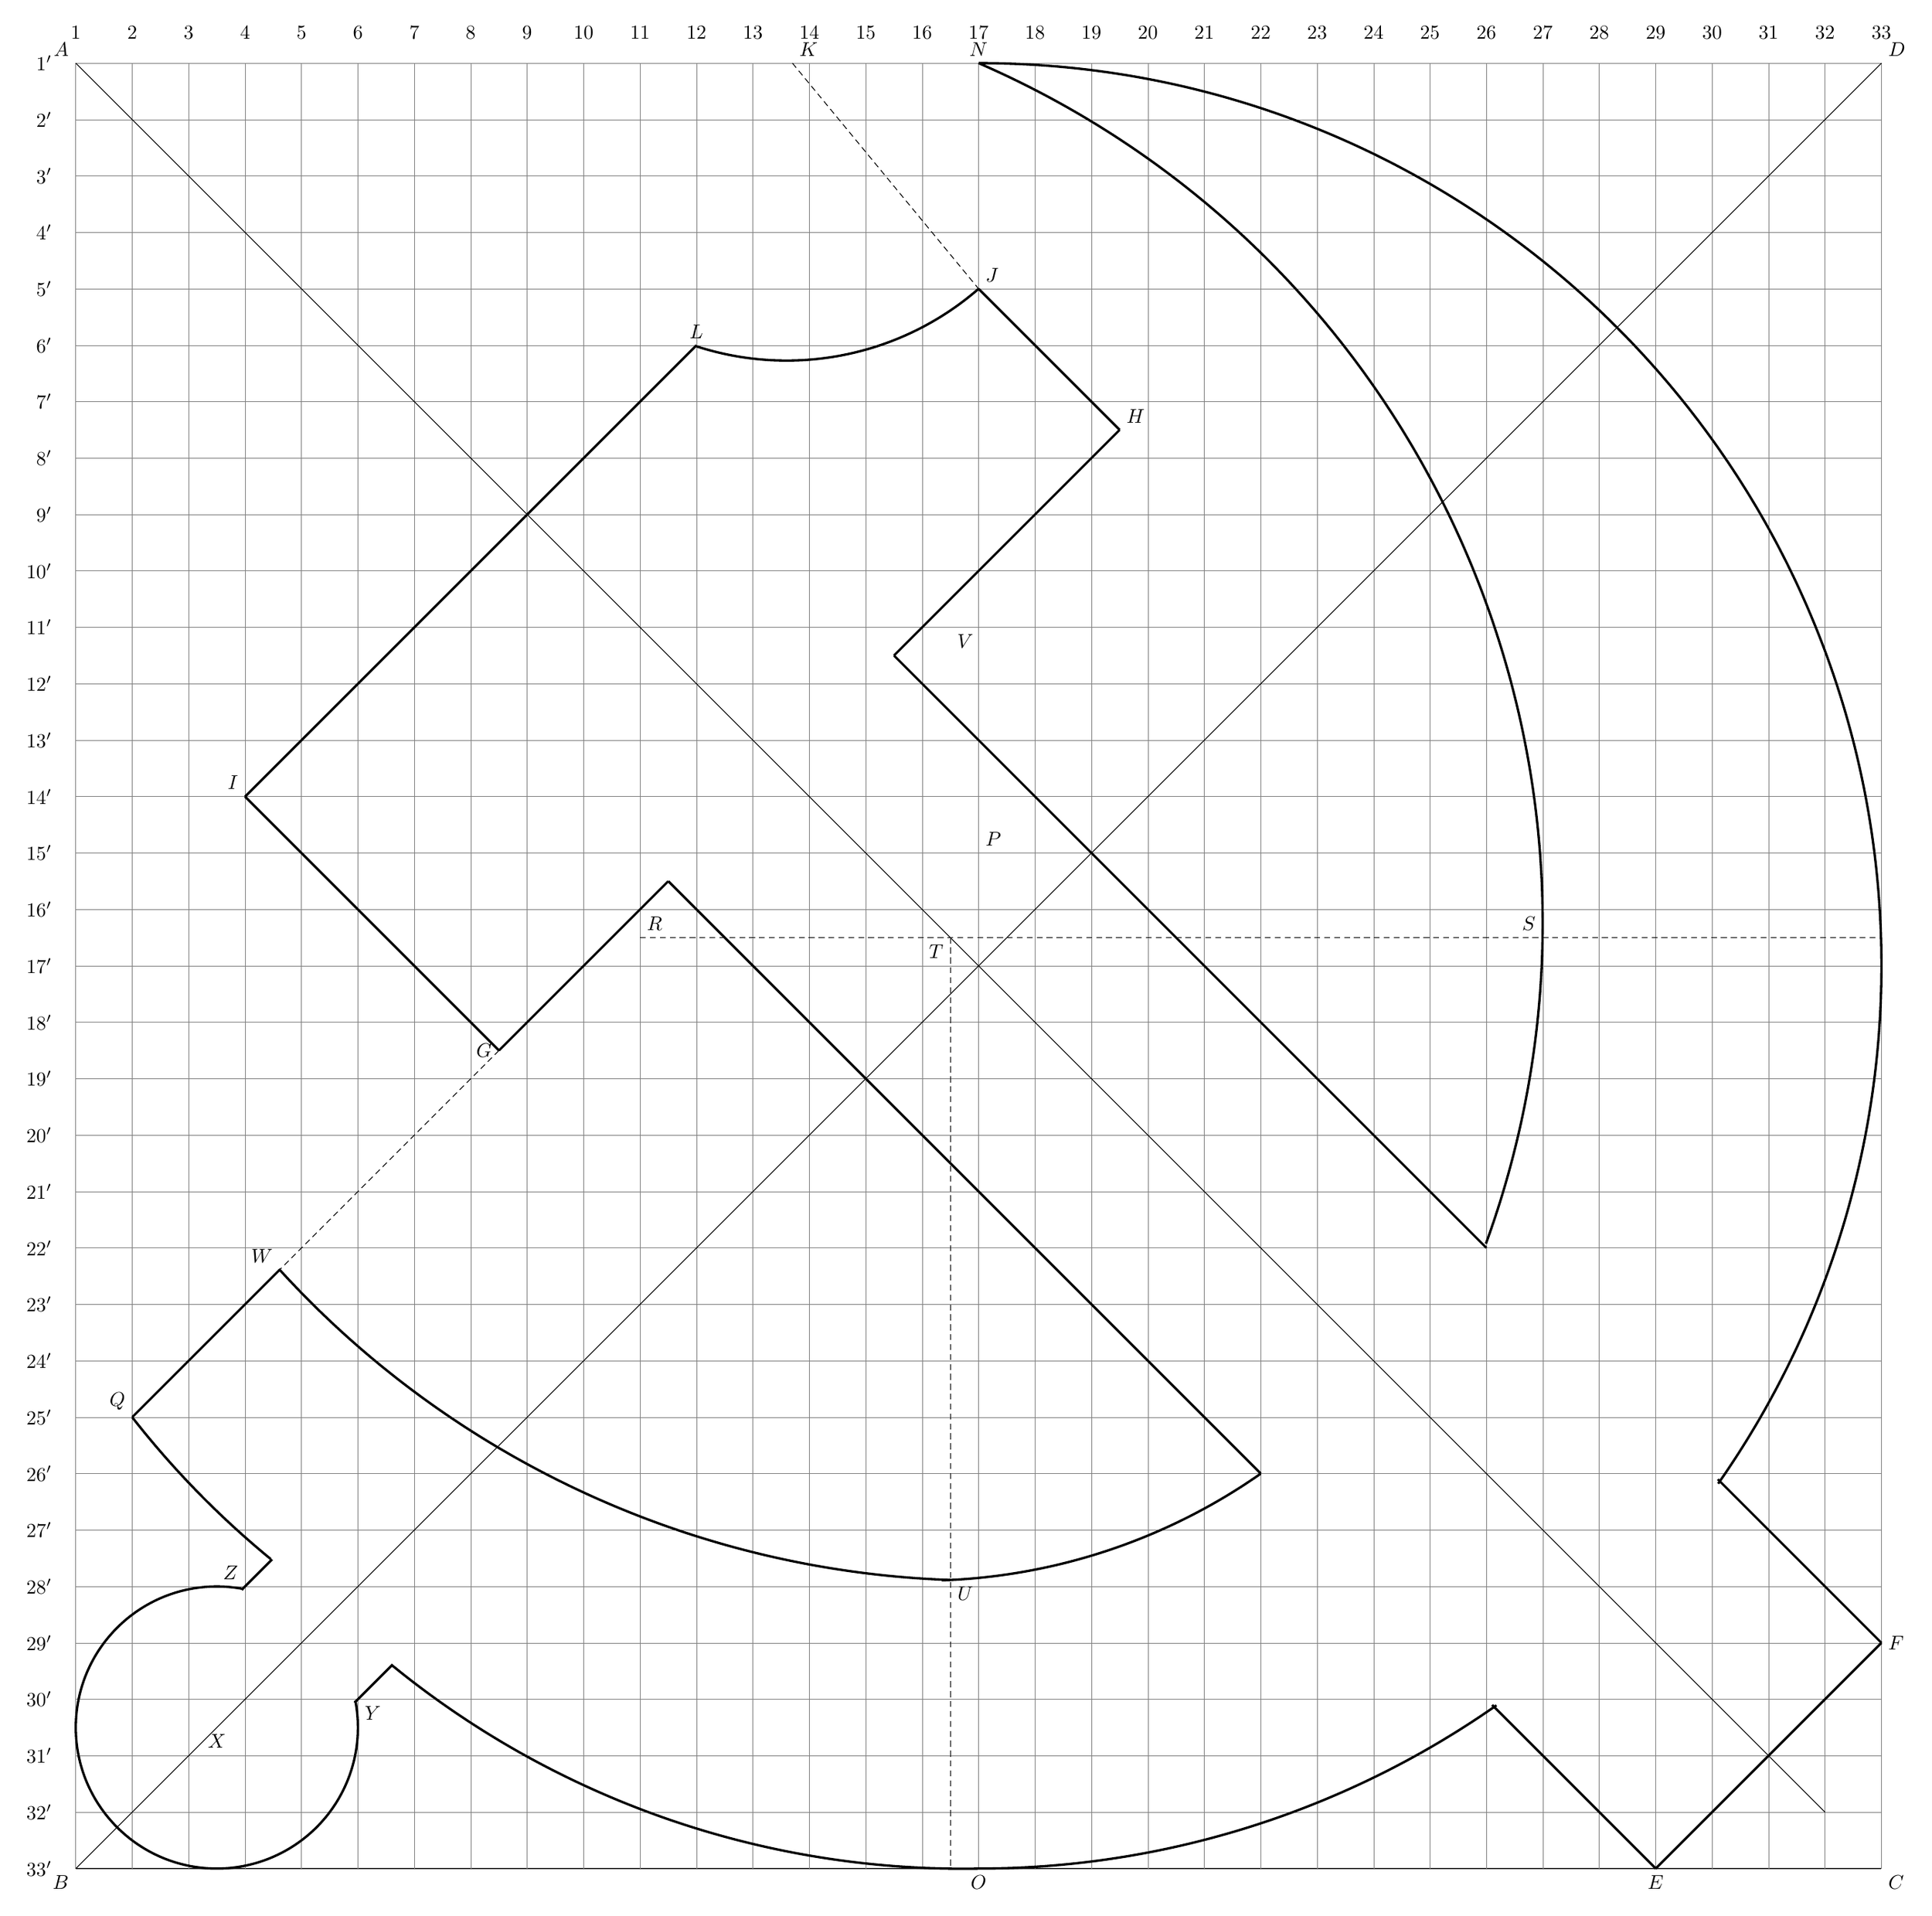
\begin{tikzpicture}[]
        % 绘制辅助线
        \draw (0,0) rectangle (32,32);
        \draw [help lines] (0,0) grid (32,32);

        % 标记坐标轴的点
        \foreach \i in {33,32,...,1}
        {
            \coordinate (\i) at ($(0,33)-(0,\i)$);
            \coordinate (\i') at ($(-1,32)+(\i,0)$);
            \coordinate [label=left:$\i'$] (\i') at ($(-.3,33)-(0,\i)$);
            \coordinate [label=above:$\i$] (\i) at ($(-1,32.3)+(\i,0)$);
        }

        % 作对角线AC, BD
        \coordinate [label=above left:$A$] (A)  at (0,32);
        \coordinate [label=below right:$C$] (C)  at (32,0);
        \coordinate [label=below left:$B$] (B)  at (0,0);
        \coordinate [label=above right:$D$] (D)  at (32,32);
        \draw [name path=AC] (A) -- (31,1);
        \draw [name path=BD] (B) -- (D);

        %%%%%% 锤头 %%%%%%%
        % 绘制锤把
        \coordinate [label=below:$E$] (E) at (28,0);
        \coordinate [label=right:$F$] (F) at (32,4);
        \draw [name path=EF, very thick] (E) -- (F);
        \draw [very thick] (E) -- (25.1,2.9);
        \draw [very thick] (F) -- (29.1,6.9);

        \draw [very thick] (21,7) -- (10.5,17.5);
        \draw [very thick] (25,11) -- (14.5,21.5);

        % 绘制锤头
        \coordinate [label=left:$G$] (G) at (7.5, 14.5);
        \coordinate [label=above right:$H$] (H) at (18.5, 25.5);
        \draw [very thick] (G) -- (10.5,17.5);
        \draw [very thick] (H) -- (14.5,21.5);
        \coordinate [label=above left:$I$] (I) at (3,19);
        \coordinate [label=above right:$J$] (J) at (16, 28);
        \draw [name path=GI, very thick] (G) -- (I);
        \draw [name path=HJ, very thick] (H) -- (J);
        \coordinate [label=above:$L$] (L) at (11,27);
        \draw [name path=IL, very thick] (I) -- (L);
        \coordinate [label=above right:$K$] (K) at (12.7, 32);
        \draw [densely dashed] (K) -- (J);
        \draw [name path=KJL, very thick]
        let 
            \p1=($(K)-(J)$),
            \n1={veclen(\x1,\y1)}
        in 
            (J) arc (-49:-108:\n1);


        %%%%%% 镰刀 %%%%%%%
        % 绘制镰刀
        \coordinate (M) at (16,16);
        \coordinate [label=above:$N$](N) at (16,32);
        \coordinate [label=below:$O$] (O) at (16,0);
        \coordinate [label=above right:$P$] (P) at (16,18);
        \coordinate [label=above left:$Q$] (Q) at (1,8);
        \draw [densely dashed, name path=GH] (G) -- (Q);
        \coordinate [label=above right:$R$] (R) at (10,16.5);
        \coordinate [label=below left:$T$] (T) at (15.5,16.5);
        \coordinate [label=below right:$V$] (V) at (15.5,22);

        \draw [very thick]
        let 
            \p1=($(M)-(N)$),
            \n1={veclen(\x1, \y1)}
        in 
            (N) arc (90:-35:\n1)
            (O) arc (270:305:\n1)
            (O) arc (271:230.7:\n1)
            (Q) arc (218:230.6:\n1);

        \draw [name path=RS,densely dashed] (R) -- (32,16.5);
        \draw [name path=RNS, very thick]
        let 
            \p1=($(R)-(N)$),
            \n1={veclen(\x1,\y1)}
        in 
            (N) arc (66.5:-20:\n1);

        \path [name intersections={of=RNS and RS}]
            coordinate [label=above left:$S$] (S) at (intersection-1);

        \draw [densely dashed, name path=TU]
            (T) -- (15.5,0);
        \draw [name path=TUS, very thick]
        let 
            \p1=($(T)-(S)$),
            \n1={veclen(\x1,\y1)}
        in 
            (21,7) arc (305:272:\n1);

        \path [name intersections={of=TUS and TU}]
            coordinate [label=below right:$U$] (U) at (intersection-1);

        \draw [name path=UVW, very thick] 
        let 
            \p1=($(U)-(V)$),
            \n1={veclen(\x1,\y1)}
        in 
            (U) arc (268:222.3:\n1);
        \path [name intersections={of=UVW and GH}]
            coordinate [label=above left:$W$] (W) at (intersection-1);
        \draw [very thick] (W) -- (Q);

        % 绘制镰刀把
        \coordinate [label=below:$X$] (X) at (2.5,2.5);
        \coordinate [label=below right:$Y$] (Y) at (5,3);
        \coordinate [label=above left:$Z$] (Z) at (3,5); 
        \draw [very thick] 
            (2.5,5) arc (90:365:2.5)
            (2.5,5) arc (90:79:2.5)
            (5,2.5) arc (0:11:2.5) 
            (2.94,4.94) -- (3.48,5.48)
            (4.94,2.94) -- (5.6,3.6);

    \end{tikzpicture}
\end{document}